Para una correcta implementaci�n del m�todo HIL, se debe tener un emulador para la planta escogido en el cap�tulo \ref{CAP:tecni} con el objetivo de hacer pruebas a un controlador real para el cual en esta secci�n se escogi� el dispositivo a utilizar. 


\section{Posibles dispositivos para dise�ar el controlador}

\subsection{Arduino Ethernet}


\begin{figure}[H]
	\centering
	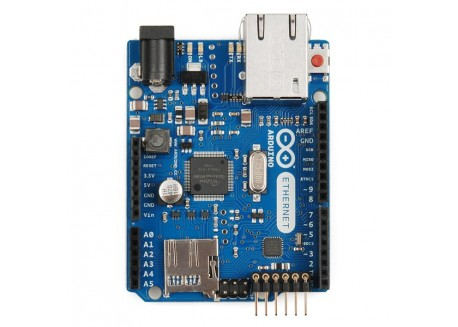
\includegraphics[width=0.7\linewidth]{img/arduinoethernet}
	\caption{Arduino Ethernet}{Fuente: https://tienda.bricogeek.com/descatalogado/392-arduino-ethernet.html}
	\label{fig:arduino}

\end{figure}

Es una placa de desarrollo Arduino con la interfaz Ethernet Wiznet que tiene las siguientes caracter�sticas:

\begin{itemize}
	\item Microcontrolador ATMega328, con frecuencia m�xima de 20 MHz.
	\item El voltaje de funcionamiento es de 5V.
	\item  El voltaje de entrada es de 7-12 V.
	\item Los puertos I/O digitales son 14 (4 cuentan con el controlador Ethernet) y 6 entradas anal�gicas.
	\item  Tiene un controlador de Ethernet integrado W5100 TCP / IP.
	\item Cuenta con una conexi�n RJ45, un conector de alimentaci�n, una cabecera ICSP y un bot�n de reinicio.
	\item Memoria de 32 KB y memoria RAM de 2KB. 
\end{itemize}
 
Este dispositivo oscila en un costo entre 45\$  y 55\$  pero el producto esta descontinuado (consultado en octubre 2021. Fuente: https://tienda.bricogeek.com/descatalogado/392-arduino-ethernet.html) y Su lenguaje de programaci�n basado en c++.

\subsection{ESP 8266}
\begin{figure}[H]
	\centering
	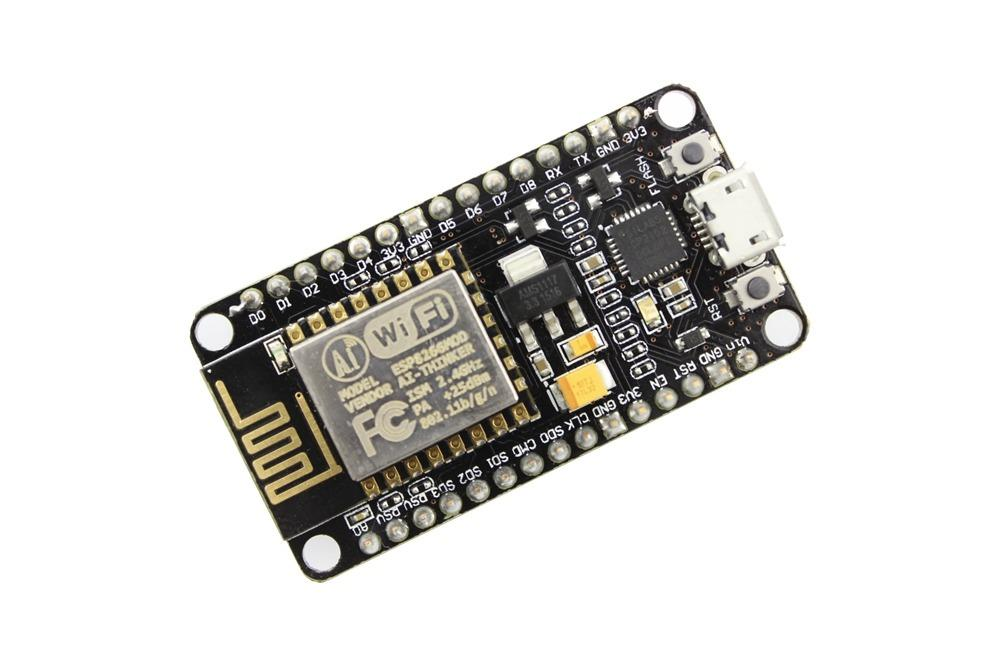
\includegraphics[width=0.7\linewidth]{img/esp8266}
	\caption{ESP 8266}{Fuente: https://sumador.com/products/modulo-wifi-esp8266-esp-12e}
	\label{fig:esp8266}
	
\end{figure}

Es un microcontrolador fabricado por Espressif Systems que tiene las siguientes caracter�sticas:

\begin{itemize}
	\item Tiene n�cleo Xtensa Tensilica L106 de 32 bit con velocidad de 80MHz.
	\item Tiene 16 GPIO (Se puede configurar entradas, salidas, UART).
	\item  Posee un pin de entrada anal�gica
	\item Tiene una memoria flash de 4 MB y 32kB de memoria RAM .
	\item  El convertidor anal�gico/digital es de 10bit.
	\item Tiene conectividad con WI-FI, pudiendo establecer servidores TCP/IP, UDP.
	\item Posee compatibilidad con SPI, I2C, I2S.
	
\end{itemize}


El dispositivo tiene un precio que varia entre los 4\$ y los 7\$ (Consultado en octubre 2021) y puede programarse en lenguaje Simba, Lua o C. 

\subsection{Rasberry Pi 3 (modelo B+)}

\begin{figure}[H]
	\centering
	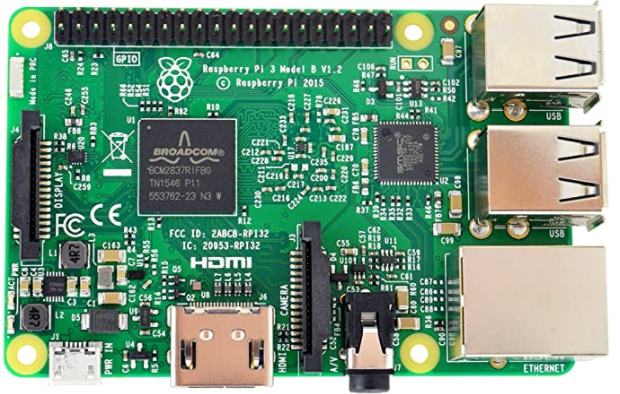
\includegraphics[width=0.7\linewidth]{img/ras}
	\caption{Rasberry Pi 3 (modelo B+)}{Fuente: https://www.raspberrypi.com/products/raspberry-pi-4-model-b/}
	\label{fig:ra}
	
\end{figure}


Es un dispositivo realizado por Raspberry Pi y cuenta con las siguientes caracter�sticas:

\begin{itemize}
	\item Microprocesador Broadcom BCM2837B0,
	propiamente un Cortex-A53 (ARMv8) de 64-bit
	\item Posee cuarenta pines de GPIO, dos UART, adem�s de cuatro puertos USB,
	un puerto HDMI, un conector auxiliar y puerto para conexi�n Ethernet.
	\item La velocidad de procesamiento es de 1.4GB.
	\item Se puede conectar memoria SD y display t�ctil.
	\item Tiene comunicaci�n Bluetooth y compatibilidad con m�dulos de conexi�n Wi-Fi.
	\item Cuenta con memoria flash de aproximadamente 1GB.
	
\end{itemize}

Este dispositivo tiene un costo entre 40\$ a 60\$ (Consultado en octubre 2021). Permite la ejecuci�n de sistemas operativos basados en Linux, es decir que puede programarse en lenguajes como Python, C$\#$ o C.



\subsection{Selecci�n}


Los puntos a considerar para la selecci�n del microcontrolador se basaron en  las siguientes caracter�sticas: costo del dispositivo, velocidad de procesamiento, memoria RAM y que posea comunicaci�n por puerto serial.

Se estima que el costo del dispositivo sea accesible para los estudiantes que necesiten utilizar el programa y de este modo puedan implementar el dispositivo real. Se necesita que la comunicaci�n entre el controlador y el emulador sea en tiempo real o con el m�nimo retardo por esto es importante saber cual es la velocidad de procesamiento del dispositivo.

Como se detallo en la secci�n  \ref{sec:diint} la comunicaci�n entre la interfaz de emulaci�n y el controlador se realiza por puerto serial por este motivo se necesita un conector de puerto USB.

La memoria RAM es la que permite cargar todas las instrucciones que se mandan entre el dispositivo y el emulador.

Para seleccionar y discriminar el dispositivo que mejor se ajusta a los requerimientos mencionados se utiliz� la figura


 
